\section{实验结果}
\subsection{实验4.1}
\begin{figure}[!htbp]
    \centering
    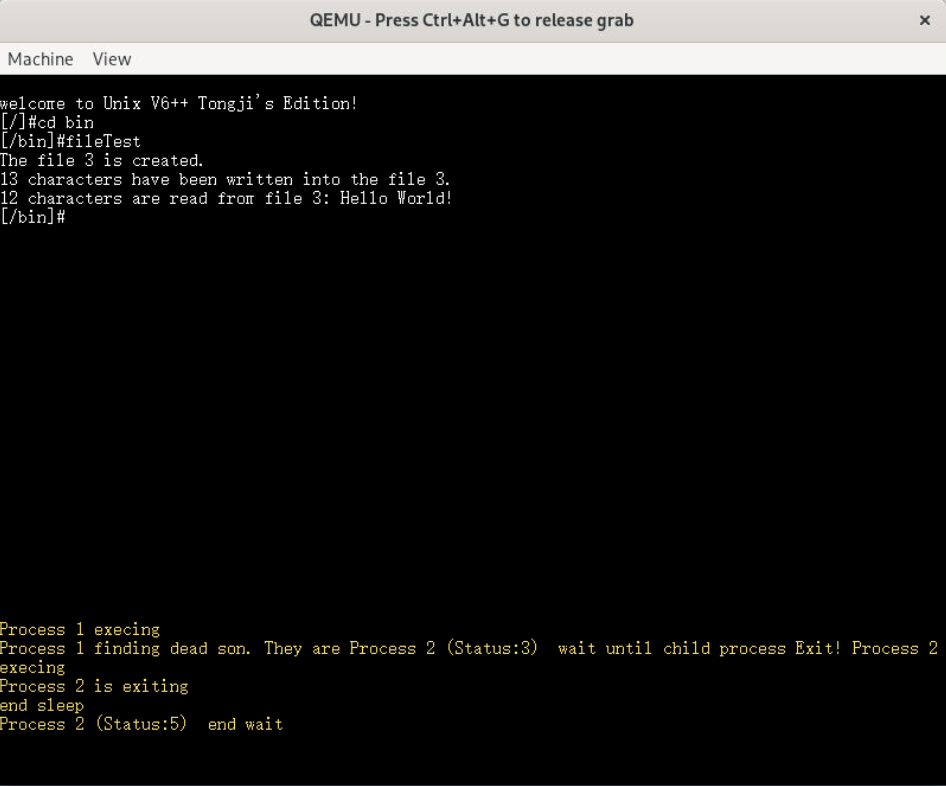
\includegraphics[width=\textwidth]{images/p1true.png}
    \caption{代码\ref{lst:fileTest}执行结果}\label{p1true}
\end{figure}

\begin{figure}[!htbp]
    \centering
    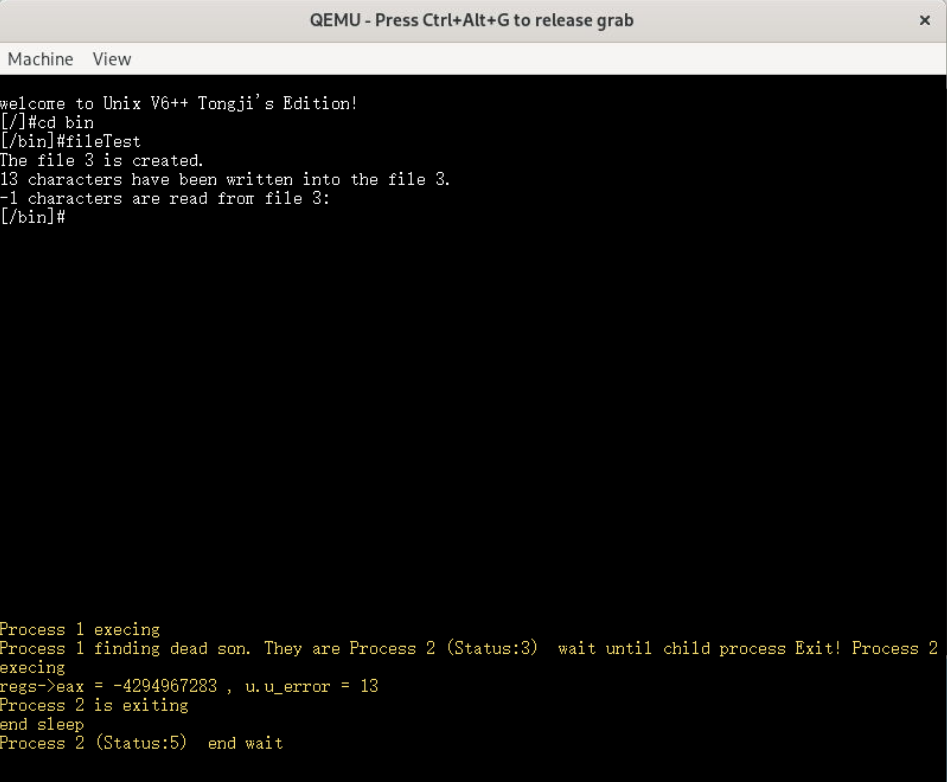
\includegraphics[width=\textwidth]{images/p1false.png}
    \caption{不重新打开文件直接读取文件的输出结果}\label{p1false}
\end{figure}

\begin{figure}[!htbp]
    \centering
    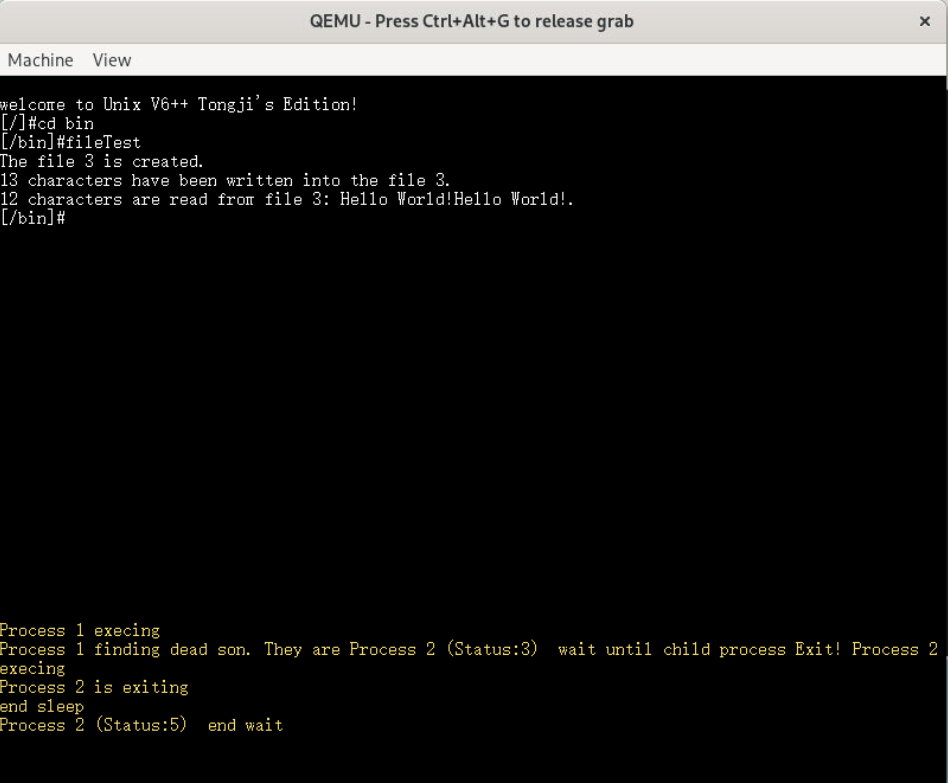
\includegraphics[width=\textwidth]{images/p112.png}
    \caption{修改字符串数组长度后的输出结果}\label{p112}
\end{figure}
\clearpage


\subsection{实验4.2}

\begin{figure}[!htbp]
    \centering
    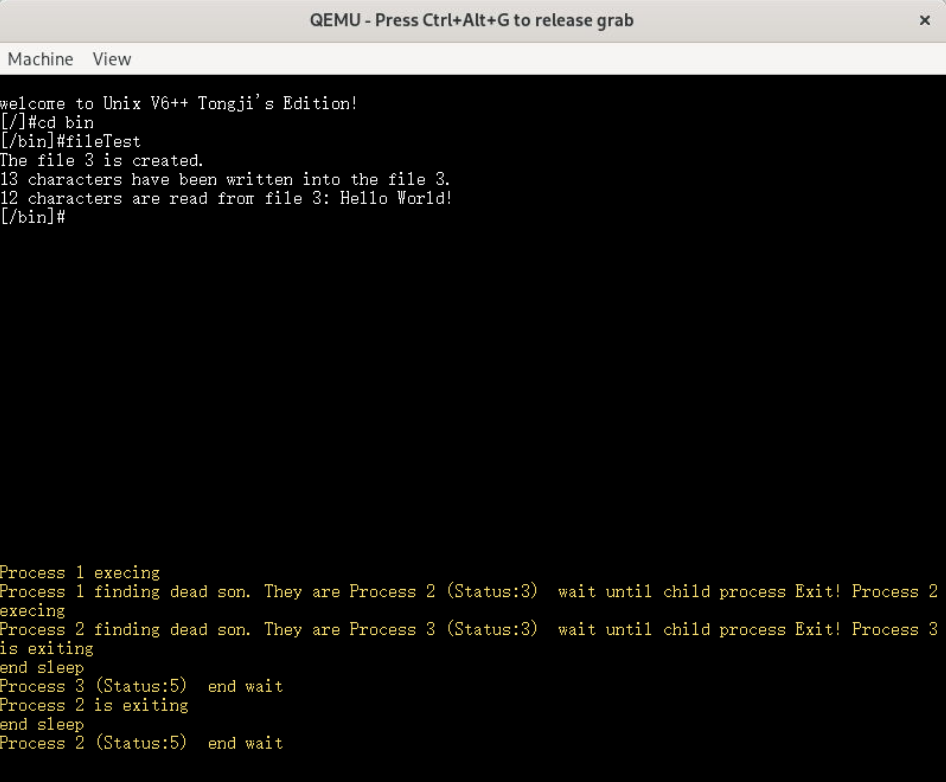
\includegraphics[width=\textwidth]{images/p2.png}
    \caption{代码\ref{lst:fileTest2}执行结果}\label{p2}
\end{figure}

\begin{figure}[!htbp]
    \centering
    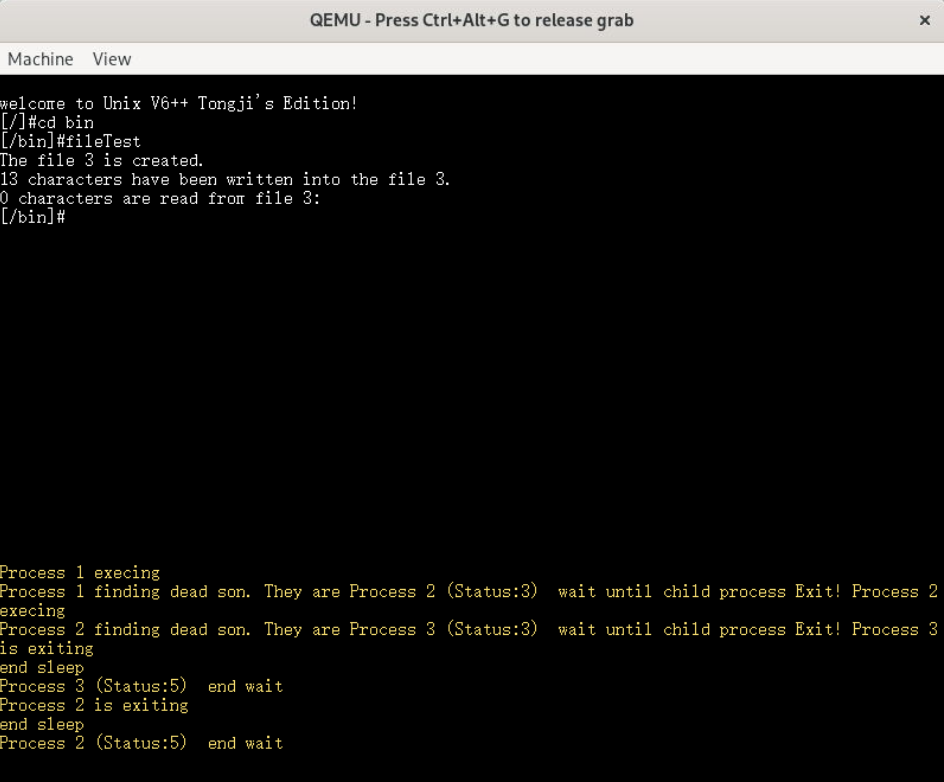
\includegraphics[width=\textwidth]{images/p2noseek.png}
    \caption{没有调用\texttt{seek}时得到的执行结果}\label{p2noseek}
\end{figure}
\clearpage
\subsection{实验4.3}
\begin{figure}[!htbp]
    \centering
    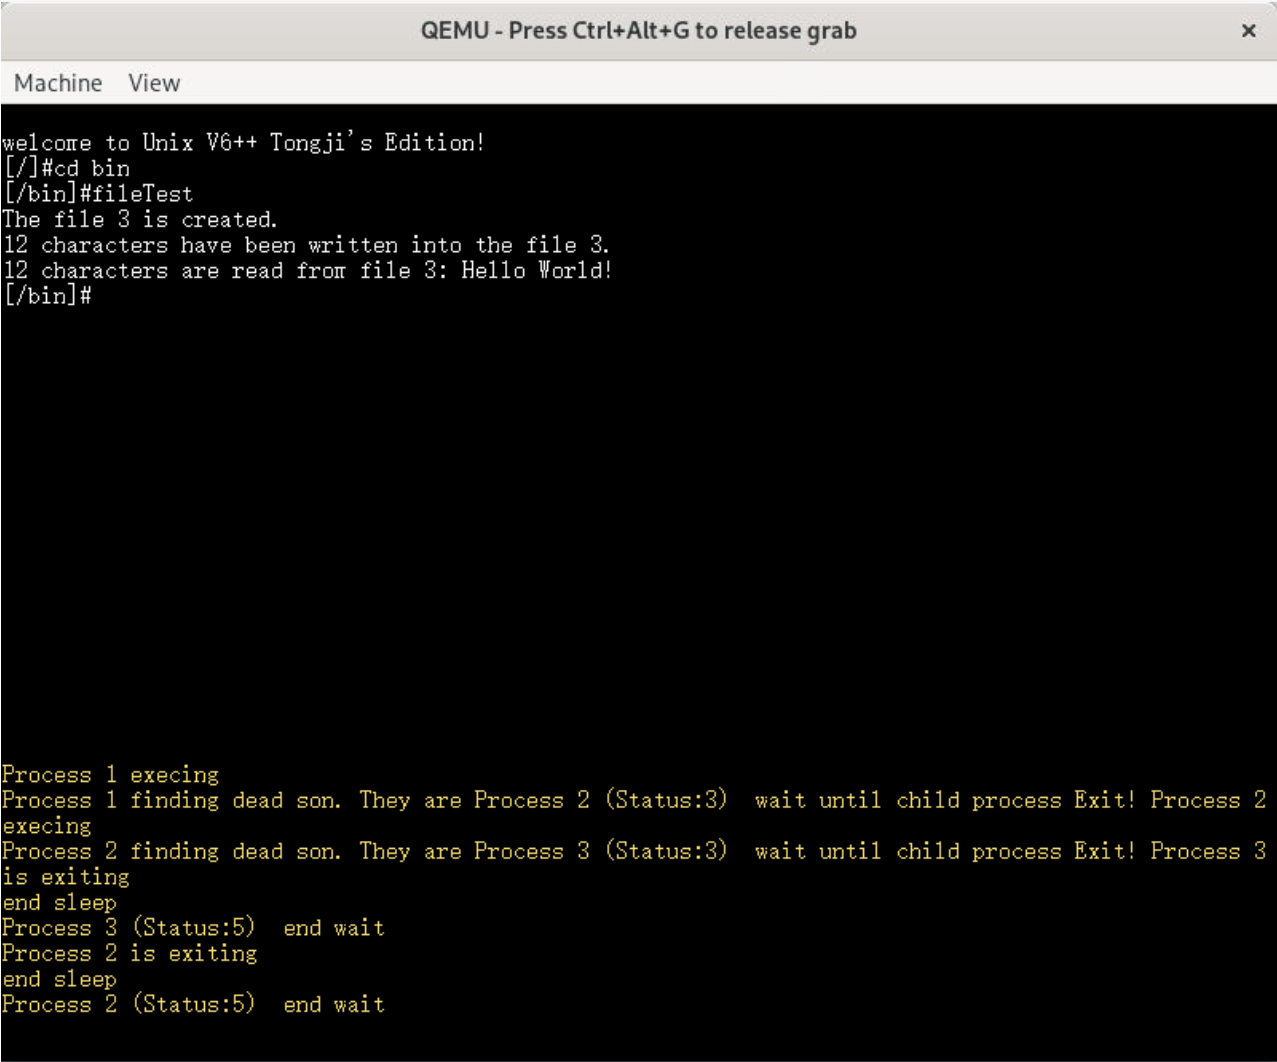
\includegraphics[width=\textwidth]{images/p3.png}
    \caption{代码\ref{lst:fileTest3}执行结果}\label{p3}
\end{figure}
